\documentclass[addpoints,10pt]{exam}

\usepackage{amsmath,amsthm,enumitem,wrapfig,amsfonts,mathtools}
\usepackage[mathscr]{euscript}
\usepackage[super]{nth}
\usepackage{dsfont}
\usepackage{xparse}
\usepackage{cancel}

\usepackage{geometry}
\usepackage[T1]{fontenc} % Use 8-bit encoding that has 256 glyphs
\renewcommand{\rmdefault}{ptm} %Change the Front Family from the default(cmr) to ptm(Times)
\usepackage{amsmath,amsfonts,amsthm,amssymb} % Math packages
\usepackage{bm}
%\usepackage{mathptmx}
\usepackage{graphicx}
\usepackage{sectsty} % Allows customizing section commands
% \allsectionsfont{\centering} % Make all sections centered, the default font and small caps

\usepackage{pgfplots}
\pgfplotsset{compat=1.18}
\usetikzlibrary{arrows.meta}
\usepackage{xcolor}
\definecolor{darkpastelgreen}{rgb}{0.01, 0.75, 0.24}
\definecolor{blue-violet}{rgb}{0.54, 0.17, 0.89}
%\usepackage{polylongdiv} %polynomial long division
% Custom problem environmenturther
\usepackage{polynom}
\newcounter{cprob}
\newenvironment{cprob}[1]{%
    \setcounter{cprob}{#1}%
    \noindent\textbf{Problem \thecprob.}%
}{%
    \par\bigskip%
}

\theoremstyle{plain}
\newcommand{\theoremname}{Theorem}
\newtheorem{thm}{\protect\theoremname}
  \theoremstyle{definition}
  \newtheorem{prob}[thm]{Problem}
  \newtheorem*{problem*}{Open Problem}
  \theoremstyle{plain}
  \newtheorem{conjecture}[thm]{Conjecture}
  \theoremstyle{plain}
  \newtheorem{lem}[thm]{Lemma}
  \newtheorem*{lem*}{Lemma}
  \newtheorem{obs}[thm]{Observation}
  \newtheorem{cor}[thm]{Corollary}
  \theoremstyle{definition}
\newtheorem{definition}[thm]{Definition}
\newcommand{\subsetdot}{\mathrel{\subset\mkern-13mu\cdot\mkern4mu}}




% Patch prob environment to be single spaced
\let\oldprob\prob
\let\endoldprob\endprob
\renewenvironment{prob}
  {\begin{singlespace}\oldprob}
  {\endoldprob\end{singlespace}}

% start problem one line below like for enumerated problems with multiple parts
\newcommand{\belowtitle}{\leavevmode\newline}
%\Observe command
\newcommand{\Observe}{\text{Observe.}}
%(=>)
\newcommand{\IF}{\mathbf{(\Rightarrow)}}
%(<=)
\newcommand{\FI}{\mathbf{(\Leftarrow)}}
%equivalence classes; \class[S]{ *content in square brackets* }
\newcommand{\class}[2][]{\ensuremath{\left[\,#2\,\right]_{#1}}}

\newcommand{\horrule}[1]{\rule{\linewidth}{#1}}
\newcommand{\kkk}{\ensuremath{\Bbbk}} 
\newcommand{\CC}{\ensuremath{\mathbb{C}}}
\newcommand{\FF}{\ensuremath{\mathbb{F}}}
\newcommand{\KK}{\ensuremath{\mathbb{K}}}
\newcommand{\NN}{\ensuremath{\mathbb{N}}}
\newcommand{\QQ}{\ensuremath{\mathbb{Q}}} 
\newcommand{\RR}{\ensuremath{\mathbb{R}}} 
\newcommand{\ZZ}{\ensuremath{\mathbb{Z}}}
\newcommand{\MM}{\ensuremath{\mathcal{M}}}
\newcommand{\TT}{\ensuremath{\mathcal{T}}}
\newcommand{\BB}{\ensuremath{\mathcal{B}}}
\newcommand{\VV}{\ensuremath{\mathcal{V}}}
\newcommand{\WW}{\ensuremath{\mathcal{W}}}
\newcommand{\UU}{\ensuremath{\mathcal{U}}}
\newcommand{\PP}{\ensuremath{\mathcal{P}}}
\newcommand{\LL}{\ensuremath{\mathcal{L}}}
\newcommand{\kk}{\ensuremath{\mathds{k}}}
\newcommand{\EE}{\ensuremath{\mathbb{E}}}
\newcommand{\A}{\ensuremath{\mathcal{A}}}
\newcommand{\YY}{\ensuremath{\mathcal{Y}}}



\newcommand{\sm}{\char`\\}
%vector stuff
\DeclarePairedDelimiter{\ip}{\langle}{\rangle} %inner product/generate
\DeclarePairedDelimiter{\norm}{\lVert}{\rVert} %norm
\DeclarePairedDelimiter{\sqb}{\lbrack}{\rbrack} %corrd

\newcommand{\floor}[1]{\left\lfloor #1 \right\rfloor}
\newcommand{\ceil}[1]{\left\lceil #1 \right\rceil}
\newcommand{\mbf}[1]{\ensuremath{\mathbf{#1}}}
\newcommand{\tbf}[1]{\textbf{ #1 }}
\newcommand{\Span}{\ensuremath{\mathrm{Span}}}
\newcommand{\Char}[1]{\mathrm{Char}\; #1}
\DeclareMathOperator{\lcm}{lcm}
\newcommand{\id}{\ensuremath{\mathrm{id}}}
\newcommand{\Gal}[2]{\mathrm{Gal}(#1/#2)}
\newcommand{\Aut}{\ensuremath{\mathrm{Aut}}}
\newcommand{\Fix}[2]{\mathrm{Fix}_{#1}(#2)}
\newcommand{\nil}{\ensuremath{\mathrm{nil}}}
\newcommand{\Hom}{\ensuremath{\mathrm{Hom}}}
\newcommand{\Obj}{\ensuremath{\mathrm{Obj}}}

\newcommand{\Rng}{\ensuremath{\mathrm{Rng}}}
\newcommand{\Ring}{\ensuremath{\mathrm{Ring}}}




\makeatletter
\renewcommand*\env@matrix[1][*\c@MaxMatrixCols c]{%
  \hskip -\arraycolsep
  \let\@ifnextchar\new@ifnextchar
  \array{#1}}
\makeatother

\def\env@matrix{\hskip -\arraycolsep
  \let\@ifnextchar\new@ifnextchar
  \array{*\c@MaxMatrixCols c}}

  \newcommand{\proj}[2]{\text{proj}_{#1}(#2)}
  

%%% Formatting: Page Header
\newcommand{\StudentName}{}
\newcommand{\AssignmentName}{Final}
\newcommand{\CourseName}{MATH 737 - Algebraic Combinatorics}


\pagestyle{headandfoot}
\runningheadrule
\firstpageheadrule
\firstpageheader{\CourseName}{\StudentName}{\AssignmentName}
\runningheader{\CourseName}{\StudentName}{\AssignmentName}
\firstpagefooter{}{\thepage}{}
\runningfooter{}{\thepage}{}

\printanswers

\DeclareMathAlphabet{\mathcal}{OMS}{cmsy}{m}{n}

\usepackage{parskip}
\usepackage{setspace}



% % % % % % % % % % % % % % % % % % % % % % % % % % % % % % % % % % % % % % % % % % % % % % % % % % % % % % % % % % % % % % 
\begin{document}

%%%%%%%%%%%%%%%%%%%%%%%%%%%%%%%%%%%%%%%%%%%%%%%%% 0 %%%%%%%%%%%%%%%%%%%%%%%%%%%%%%%%%%%%%%%%

\setcounter{thm}{0}
\renewcommand{\thethm}{5.\arabic{thm}}
 % next prob is 5.1

%%%%%%%%%%%%%%%%%%%%%%%%%%%%%%%%%%%%%%%% Sagan Ch. 5 %%%%%%%%%%%%%%%%%%%%%%%%%%%%%%%%%%%%%%%
\begin{center}
    \underline{\textbf{Exercises}}
\end{center}
Recall the definition of a $\sigma^{+-}$-labeling of a graph $G$ on $m$ edges.
\begin{definition}
    The length of a $\ZZ$-labeled edge $ab$ modulo $n$ is defined by $\ell_{n}(ab)=\min\{n-|a-b|,|a-b|\}$. We call an injection $f:\{0,1,\hdots,2m-2\}\hookrightarrow V(G)$ a $\sigma^{+-}$-labeling of a graph $G$ on $m$ edges if
    \begin{enumerate}
        \item $f(V(G))=A\sqcup B$ such that $ab\in f(E(G))\implies a<b$; All neighbors of each $v\in f(V(G))$ are either bigger or smaller than $v$
        \item Every edge is a short edge: $\ell(ab)=|a-b|,\forall ab\in f(E(G))$ and there is exactly one edge of each length in $\{1,\hdots, m\}$
        \item The edge of length $m$ is a \textit{pendant edge} which means one of it's endpoints has only one neighbor; it is incident to a leaf.
    \end{enumerate}
\end{definition}

$\ZZ_{n}$ acts on the set of all $\ZZ-$labeled subgraphs $S(K_{n})$ of $K_{n}$ in the following way for each $H\in S(K_{n})$ and each $g\in \ZZ_{n}$: 
$$g(H)\coloneq\text{ the subgraph induced by }V(H)+g\pmod{n};\text{ just add g to every vertex}$$

\begin{prob}
$\newline$
    \begin{enumerate}
        \item Find a $\sigma^{+-}$-labeling of $S_{4}\sqcup P_{1}$. (lengths should be $1-4$, labels should be $\{0,1,\hdots, 6\}$)
        \item Find it's orbit via the $\ZZ_{9}$ action.
    \end{enumerate}
\end{prob}

\begin{center}
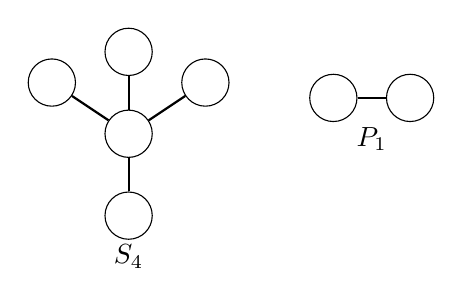
\begin{tikzpicture}[
    scale=.65,every node/.style={circle, draw, minimum size=6mm, inner sep=0pt},
    edge/.style={thick}
]
    % S_4
    \node (c) at (0,0) {};
    \node (a) at (-1.5,1) {};
    \node (b) at (0,1.6) {};
    \node (d) at (1.5,1) {};
    \node (e) at (0,-1.6) {};

    \draw[edge] (c)--(a);
    \draw[edge] (c)--(b);
    \draw[edge] (c)--(d);
    \draw[edge] (c)--(e);

    % P_1
    \node (p) at (4,0.7) {};
    \node (q) at (5.5,0.7) {};

    \draw[edge] (p)--(q);

    \node[draw=none] at (0,-2.4) {$S_4$};
    \node[draw=none] at (4.75,-0.1) {$P_1$};
\end{tikzpicture}
\end{center}

\begin{center}
    %%%%%%%%%%%%%%%%%%%%%%%%%%%%%%
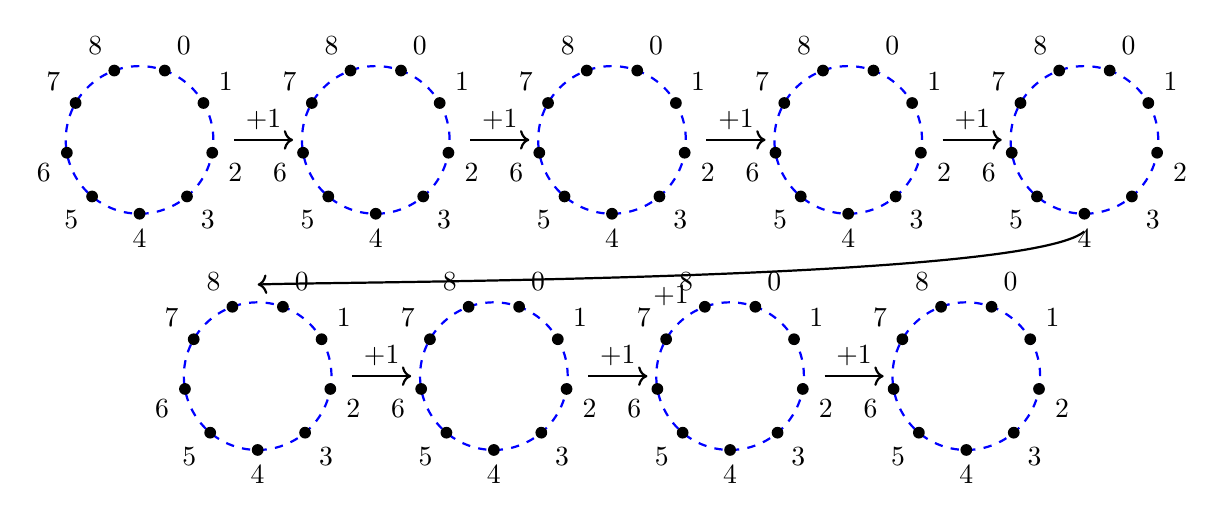
\begin{tikzpicture}[
    scale=.75,
    vertex/.style={circle, fill=black, inner sep=1.5pt},
    orbit/.style={blue, dashed, thick},
    shiftarrow/.style={->, thick}
]

\newcommand{\blankKnine}[2]{%
    \begin{scope}[shift={(#1,#2)}]
        \draw[orbit] (0,0) circle (1.25);
        \foreach \i in {0,...,8}{
            \node[vertex,label={{{70-40*\i}}:$\i$}] at ({70-40*\i}:1.25) {};
        }
    \end{scope}
}

% top row: 5 copies
\blankKnine{0}{0}
\blankKnine{4}{0}
\blankKnine{8}{0}
\blankKnine{12}{0}
\blankKnine{16}{0}

% bottom row: 4 copies
\blankKnine{2}{-4}
\blankKnine{6}{-4}
\blankKnine{10}{-4}
\blankKnine{14}{-4}

% arrows top row
\foreach \x in {1.6,5.6,9.6,13.6}{
    \draw[shiftarrow] (\x,0) -- ++(1,0) node[midway, above] {$+1$};
}

% wrap arrow
\draw[shiftarrow] (16,-1.55) .. controls (15,-2.4) and (3,-2.4) .. (2,-2.45)
    node[midway, below] {$+1$};

% arrows bottom row
\foreach \x in {3.6,7.6,11.6}{
    \draw[shiftarrow] (\x,-4) -- ++(1,0) node[midway, above] {$+1$};
}

\end{tikzpicture}
\end{center}

%%%%%%%%%%%%%%%%%%%%%%%%%%%%%%%%%%%%%%%%%%%%%%%% 5.1 %%%%%%%%%%%%%%%%%%%%%%%%%%%%%%%%%%%%%%%


\end{document}